% !TeX encoding=utf8
% !TeX spellcheck = de-DE

\chapter{Applikation}



Vorsichtsmassnahme, dass gewisse Ameisen sterben (weil z.B. 500 Ameisen, die sich auf einer Seite des Displays befinden, nicht zurück können, da sie den Weg zurück nicht nehmen können; sobald ein bester Pfad gefunden ist, sterben gewisse Ameisen nach einer gewissen Zeit, wenn sie nicht mehr mit Pheromon in Verbindung kommen) \\


\section{Aufbau/Überblick}

Struktur des Programms beschreiben \\


\vspace*{1cm}

\subsection{Pygame (Sprites)}


\vspace*{1cm}


\subsection{Graph: Datenstruktur (Gründe für deren Verwendung)}


\vspace*{1cm}



\section{Mockups}

Zwei verschiedene Varianten für das spätere Aussehen des Programms standen im Vordergrund: eine mit der Einstellungsleiste im oberen Fensterbereich, eine zweite mit den Einstellungen am rechten Seitenrand.


\begin{figure}[h]
  \centering
	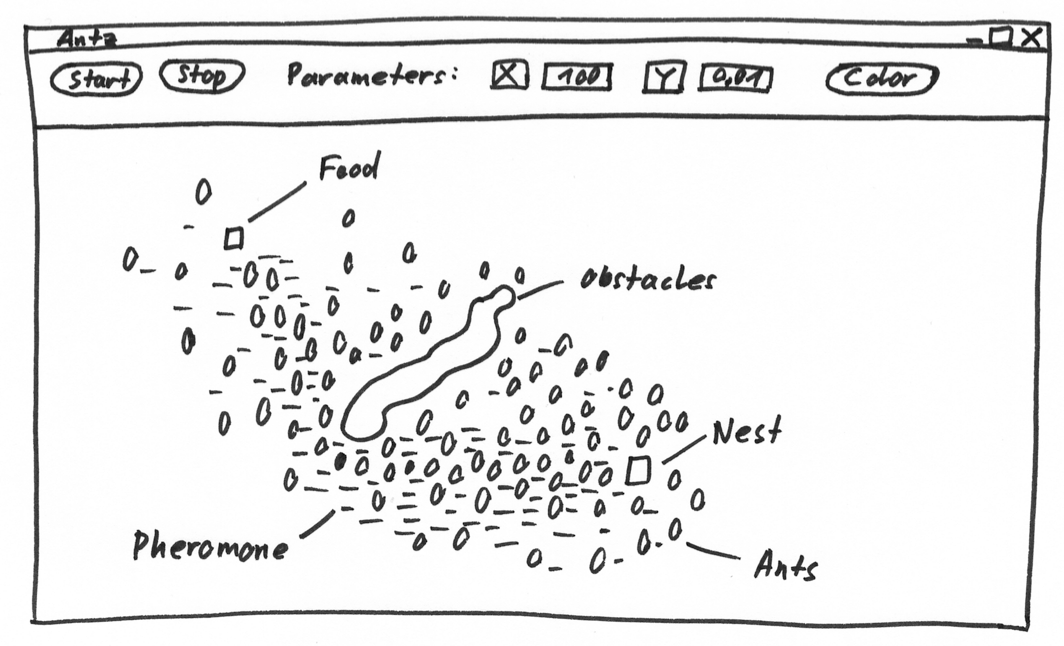
\includegraphics [width=0.85\textwidth]{images/Antz_Mockup_1_sw.png} 
	\caption{Mockup-Variante 1: Einstellungen im oberen Fensterbereich}
\end{figure}


%\begin{minipage}[h]{10cm}
%\vspace*{2.5cm}
%\end{minipage}


\begin{figure}[h]
  \centering
	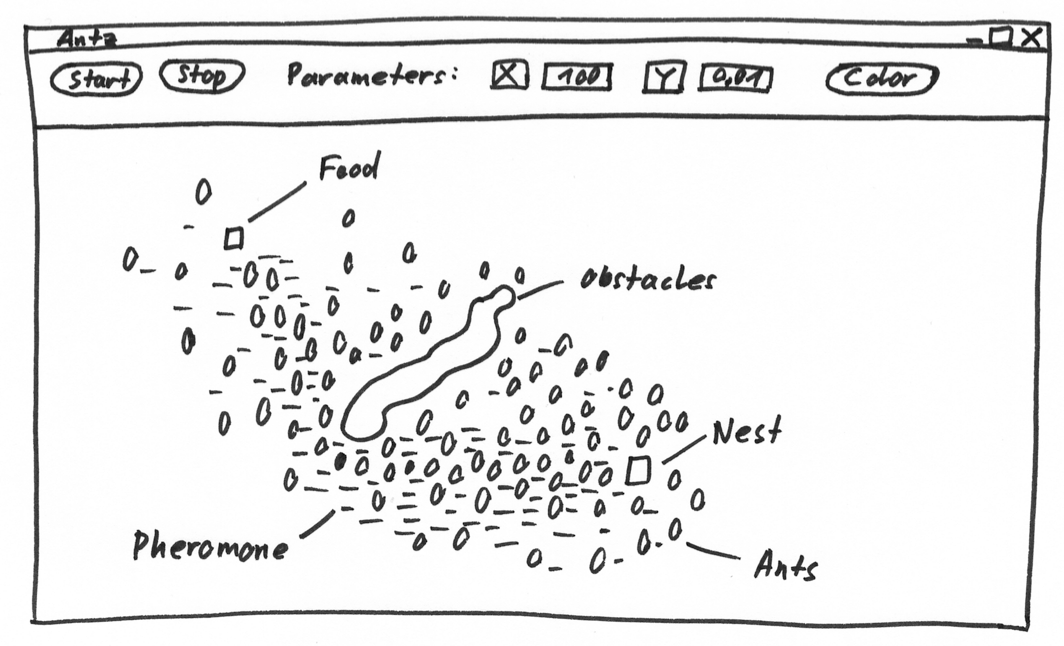
\includegraphics [width=0.85\textwidth]{images/Antz_Mockup_1_sw.png} 
	\caption{Mockup-Variante 2: Einstellungen im rechten Fensterbereich}
\end{figure}


\vspace*{2cm}



\section{Klassendiagramme}


\vspace*{1cm}


\section{Screenshots aus dem Programm}


\vspace*{1cm}


\section{Auswertungen: Konvergenz, Parameter}


\vspace*{1cm}


\section{Algorithmus/Performance, gewichtete Wahrscheinlichkeiten}


\vspace*{1cm}


\subsubsection*{Iteration 1}

Noch nicht implementiert, dass die Wegfindung abhängig von der Anzahl Ameisen, die durchlaufen, ist. \\

Evtl. noch eine Multi-Threaded-Lösung integrieren (sehr gut zu parallelisieren) \\

Ausserdem: schnellere Python-Interpreter wie pypy (oder für numerische Berechnungen); für z.B . 10'000 Nodes! \\

Idee: vielleicht noch Rauschen integrieren? Random von 20\,\% konvergiert überhaupt nicht mehr.

\vspace*{3cm}


Inputs von Syrus: \\

\begin{itemize}
\item Interessant wäre, das Maximum der Verlangsamung bei mehr Ameisen zu messen
\item Eventuell in Richtung Programming Tuning gehen? (Performance-Messungen: wie viel fällt auf welchen Bereich?) 
\item Für die Iterationen 2 und 3: Einsatz der Ressourcen planen (Andere Algorithmen; Optimierung; Vergleich mit Djikstra: Statistiken; vgl. Optimierungspotential bezüglich Zeit und Speicheraufwand, etc.); z.B. eher TSP (weil visuell für die Mitstudierenden ansprechender?) 
\end{itemize}